\chapter{The 2-dimensional model with migration}\label{ch:4_2D_model}

In Chapters~\ref{ch:2_base_model} and \ref{ch:3_2Lvl_model}, we examined the evolution of cooperation under environmental variability (EV) using models with explicit group structures.
The base model in Chapter~\ref{ch:2_base_model} demonstrated that EV can promote cooperation without migration.
The 2-level model with migration in Chapter~\ref{ch:3_2Lvl_model} extended this by introducing individual-level migration and demonstrated that EV can still promote cooperation.
Moreover, moderate migration promotes cooperation while excessive migration hinders it.
However, the 2-level model is relatively unique and limits clear comparison with existing studies on cooperation and migration.
In this chapter\protect\footnote{This chapter is based on Inaba and Akiyama (2025) \cite{Inaba2025b}, published in \textit{Chaos, Solitons \& Fractals}.}, we adopt a 2-dimensional (2D) space, which is widely used in the literature, diverging from the group-structured frameworks of Chapters \ref{ch:2_base_model} and \ref{ch:3_2Lvl_model} to prioritize comparability with prior works.

The evolution of cooperation among mobile agents has been studied actively.
Dugatkin and Wilson (1991) \cite{Dugatkin1991} performed pioneering work in this area, demonstrating that the effectiveness of Axelrod's Tit-for-Tat strategy \cite{Axelrod1981} can be undermined by mobile defectors (Rover strategy) when migration costs are low, although their model employed a patch structure rather than a 2D space.
More contemporary research in 2D spatial settings, where both cooperators and defectors can migrate, was initiated by Vainstein and Arenzon (2001) \cite{Vainstein2001} and established by Vainstein et al. (2007) \cite{Vainstein2007}.
They demonstrated that mobility can have contrasting effects: under certain conditions, it promotes cooperation by facilitating cooperator clustering and separation from defectors, while under other conditions, it hinders cooperation by generating strategic chaos.
These developments are reviewed in Perc and Szolnoki (2010) \cite{Perc2010}.
Building on Vainstein's framework, various migration strategies \cite{Cong2012, Chen2012, He2020, Dhakal2020, Ren2021, Yang2023, Zhang2025} differing in trigger conditions and migration distance have been proposed more recently.
However, to the best of our knowledge, no study has examined the effects of extrinsic EV on the evolution of cooperation among mobile agents.

This chapter addresses this gap within Vainstein's framework by modeling EV as randomly moving resource-rich spots (Sources of Resources; SoRs) across a 2D space and agent mobility as resource-seeking migration.
Through extensive simulations, we examine whether and how these factors jointly promote cooperation.

\section{Model}\label{sec:4_model}

In this chapter, we developed a multiagent simulation model to examine how agent mobility and EV jointly influence the evolution of cooperation in spatially structured populations.
Due to the limited availability of archaeological data on spatial resource distributions and hominin behavioral patterns during the MSA, we adopted an abstracted approach that prioritizes the identification of fundamental mechanisms over reproducing specific historical scenarios.
This model incorporates four key processes, i.e.,
(i) EV on a 2D lattice,
(ii) pairwise game interactions,
(iii) conditional agent migration driven by resource availability, and
(iv) strategy updating.
These processes are described in the following subsections.

\subsection*{Environmental variability}

The spatial structure is represented by a 2D lattice with periodic boundary conditions.
Here, $N$ agents are distributed randomly across the cells, and each cell contains at most one agent.
Each cell maintains a resource level that varies both spatially and temporally.
We define a Source of Resources (SoR) as a focal point that generates spatial resource gradients in the environment, and these SoRs serve as simplified representations of the natural foraging areas commonly found near rivers, lakes, and coastlines.
Each SoR creates a gradient where resource availability typically decreases with increasing distance from the SoR.
In addition, multiple SoRs may coexist, thereby forming overlapping zones of resource abundance.

In this model, each agent accumulates resources (represented by the agent's fitness value) through interactions, and local prosperity is defined by a resource threshold $\theta_{x,y}$ for each cell $(x, y)$, where $0 \leq \theta_{x,y} \leq 1$.
Agents with fitness values that are less than the threshold $\theta_{x,y}$ are more likely to migrate and update their strategies, and agents with fitness values greater than the threshold remain unchanged.
Therefore, locations with lower thresholds impose less pressure for behavioral change, indicating that these locations are prosperous and rich in resources.
Here, the threshold $\theta_{x,y}$ is determined by the cumulative influence of all SoRs and is calculated as follows:
\begin{equation}
\theta_{x,y} = \frac{D_{x,y} - D_{\min}}{D_{\max} - D_{\min}}, \quad D_{x,y} = \sum_{i=1}^{n_{SoR}} d_{x,y}^{(i)}
\end{equation}
where $n_{SoR}$ denotes the number of SoRs, $d_{x,y}^{(i)}$ denotes the Euclidean distance from cell $(x, y)$ to the $i$-th SoR, calculated under periodic boundary conditions, and $D_{\min}$ and $D_{\max}$ denote the minimum and maximum values of $D_{x,y}$ across the entire grid, respectively.

We examine two spatial configurations, which we refer to as 1-SoR and 2-SoR.
In the 1-SoR configuration (a $200\times200$ grid), a single SoR generates a concentric resource gradient, capturing the essential geographical pattern of an oasis-like environment (Figure~\ref{fig:ev}a).
In the 2-SoR configuration (a $400\times200$ grid), two SoRs generate a corridor of resource gradient, capturing the essential geographical pattern of riverine or coastal environments where resources are distributed along a line (Figure~\ref{fig:ev}b).

\begin{figure}[!ht]
\centering
\includegraphics[width=1.0\linewidth]{figures/4/Fig1.png}
\caption[Spatially heterogeneous prosperity patterns generated by SoR(s)]{
Spatially heterogeneous prosperity patterns generated by SoR(s).
The colors indicate the resource threshold $\theta_{x,y}$.
(a) A single SoR located at $(100, 100)$ on a $200\times200$ grid generates a concentric resource gradient.
(b) Two SoRs located at $(100, 100)$ and $(300, 100)$ on a $400\times200$ grid generate a band-shaped resource gradient.
(c) and (d) Examples of the stochastic movement of SoRs that dynamically reshapes the resource landscapes.
}\label{fig:ev}
\end{figure}

EV is modeled through the stochastic movement of SoRs, reflecting the unpredictable nature of the landscape dynamics observed during the MSA in Africa.
Each SoR moves to a randomly selected adjacent cell within the Moore neighborhood with a probability $p_{EV} \, (0 \leq p_{EV} \leq 1)$ at each time step, and the direction is selected uniformly at random from the eight neighboring cells.
In this process, the parameter $p_{EV}$ governs the intensity of the EV, where $p_{EV} = 0$ corresponds to a static environment, and higher $p_{EV}$ values represent more intense EV.

Throughout this chapter, the neighborhood is defined as the Moore neighborhood (i.e., eight neighboring cells).
This choice better approximates the continuous spatial movement of SoRs and mobile agents than the von Neumann neighborhood (i.e., four orthogonal cells), where movement is restricted to only cardinal directions.
In addition, for distance calculations, particularly when determining resource gradients from SoRs, the Euclidean distance is employed to produce smooth, circular gradients that better represent natural resource distributions than other metrics, e.g., the Manhattan or Chebyshev distances.

\subsection*{Game}

Games represent cooperative or competitive interactions between agents that involve the gain or loss of resources.
Each agent holds a strategy, either cooperation ($C$) or defection ($D$), which determines its behavior in interactions.
In every time step, each agent plays pairwise games with all its neighbors and accumulates a payoff $\pi_j$, which is then converted into fitness $\omega_j$ ($j \in [1,\ldots,N]$, $0 < \omega_j < 1$), representing the agent's resource level.

The payoff matrix of the game is defined as follows:
\begin{equation}
\begin{array}{c|cc}
  & C & D \\
\hline
C & R & S \\
D & T & P
\end{array}
\end{equation}
where $R = 1$, $0 < T < 2$, $-1 < S < 1$, and $P = 0$.
To ensure the robustness of the results across a range of social dilemma contexts, we consider various game structures, including the Prisoner's Dilemma ($T > R > P > S$), Stag Hunt ($R > T > P > S$), and Snowdrift ($T > R > S > P$) games.

The accumulated payoff $\pi_j$ is transformed into the fitness $\omega_j$ using a sigmoid function as follows:
\begin{equation}
\omega_j = \frac{1}{1 + \exp(-k(\pi_j - \pi_0))}
\end{equation}
where $k$ determines the steepness of the sigmoid curve, and $\pi_0$ sets the baseline payoff at which $\omega_j = 0.5$.
Here, we set $k = 1$ for moderate sensitivity and set $\pi_0 = 4.0$ to center the sigmoid around common payoff values found in mixed-strategy populations.
Given that each agent can accumulate payoffs from up to eight of its neighbors, the theoretical payoff range is $8S$ to $8R$ and $8P$ to $8T$ for cooperators and defectors, respectively.
With our parameter constraints, this yields a payoff range of $-8 < \pi_j < 16$.

\subsection*{Migration}

At each time step, agents migrate if their fitness $\omega_j$ is less than the resource threshold $\theta_{x,y}$ at their current location.
Any agent that meets this condition migrates with probability $p_M$ and remains at the location with the complementary probability $1 - p_M$.
The migration direction follows a resource-oriented bias, where an agent moves toward a neighboring cell with the lowest $\theta_{x,y}$ value with probability $p_{SoR}$ (SoR orientation) and moves randomly within the neighborhood with the complementary probability $1 - p_{SoR}$.
Cells occupied by other agents are excluded from the candidate destinations.
The agents migrate asynchronously in a randomized order to avoid movement conflicts.

\subsection*{Strategy update}

At each time step, agents update their strategies synchronously if their fitness $\omega_j$ is less than the resource threshold $\theta_{x,y}$.
Any agent that meets this condition adopts the strategy of the most successful neighbor (i.e., the neighbor with the highest fitness).
This process is subject to mutation, where the adopted strategy is replaced by the opposite strategy (e.g., from $C$ to $D$ or vice versa) with probability $\mu$.

We note that asynchronous updating \cite{Huberman1993, Zhang2025a} is more realistic and the choice of updating protocol can significantly affect outcomes in densely packed models \cite{Huberman1993}.
However, unlike densely connected lattice models where agents interact with many neighbors simultaneously, our agents typically interact with only a few neighbors on each resource patch.
This sparsity reduces the interdependence between neighboring strategy updates, making the dynamics largely insensitive to the updating protocol.

\subsection*{Evaluation}

To investigate the effects of EV and agent mobility on the evolution of cooperation, simulations are performed under a range of parameter configurations, as shown in Table~\ref{tab:4_params}.

Each configuration is evaluated through $100$ independent trials of $10000$ generations each.
As the primary outcome measure, we compute the cooperation rate $\phi_C$, which is defined as the average proportion of agents employing the $C$ strategy at the end of each generation (following the strategy update process), averaged over both the final $5000$ generations and all $100$ independent trials.

\begin{table}[!ht]
\centering
\caption[Model parameters used in the simulations]{Model parameters used in the simulations.}
\label{tab:4_params}
\begin{tabular}{cp{0.6\textwidth}p{0.2\textwidth}}
\toprule
\textbf{Parameter} & \textbf{Description} & \textbf{Value options} \\
\midrule
$W \times H$ & Grid dimensions & $200 \times 200, 400 \times 200$ \\
$N$ & Number of agents & $\{500, 1000, 2000,$ $4000, 8000, 16000\}$ \\
$\phi_C^0$ & Initial frequency of cooperators & $\{0, 0.5, 1\}$ \\
\addlinespace
$n_{SoR}$ & Total number of SoRs & $\{1, 2\}$ \\
\addlinespace
$p_{EV}$ & Probability of SoR shift; controlling the intensity of EV (shift range of the SoR, $\sigma_R$, in Chapter~\ref{ch:2_base_model}) & $\{0, 0.1, \ldots, 1\}$ \\
\addlinespace
$R$ & Payoff for mutual cooperation & $1$ \\
$T$ & Payoff for defection against cooperator & $\{0, 0.1, \ldots, 2\}$ \\
$P$ & Payoff for mutual defection & $0$ \\
$S$ & Payoff for cooperation against defector & $\{-1, -0.9, \ldots, 1\}$ \\
\addlinespace
$p_M$ & Direct probability of migration for agents below threshold (multiplied by resource deficit in Chapter~\ref{ch:3_2Lvl_model}) & $\{0, 0.1, \ldots, 1\}$ \\
\addlinespace
$p_{SoR}$ & Probability of migrating toward SoR & $\{0, 0.1, \ldots, 1\}$ \\
\addlinespace
$\mu$ & Mutation probability in strategy update & $\{0, 0.01\}$ \\
\bottomrule
\end{tabular}
\end{table}

\section{Results}\label{sec:4_results}

\subsection*{Influence of environmental variability and agent mobility}\label{sec:4_key_results}

Figure~\ref{fig:4_key_result} shows the combined effects of EV ($p_{EV}$) and agent mobility ($p_M$) on the cooperation rate $\phi_C$.
As can be seen, in stable environments ($p_{EV} = 0$) or with low agent mobility ($p_M \lesssim 0.2$), cooperation fails to evolve.
In contrast, with sufficient agent mobility ($p_M \gtrsim 0.2$), even modest EV ($p_{EV} = 0.1$) promotes cooperation; however, further variability ($p_{EV} > 0.1$) does not enhance cooperation.
In addition, agent mobility promotes cooperation with any level of EV ($p_{EV} > 0$).

\begin{figure}[!ht]
\centering
\includegraphics[width=0.7\linewidth]{figures/4/Fig2.png}
\caption[Influence of environmental variability ($p_{EV}$) and agent mobility ($p_M$) on the cooperation rate ($\phi_C$)]{
Influence of EV ($p_{EV}$) and agent mobility ($p_M$) on the cooperation rate ($\phi_C$).
The figure shows that cooperation emerges only when both $p_{EV} \gtrsim 0.1$ and $p_M \gtrsim 0.2$, with neither factor alone being sufficient to promote cooperation.
Each cell shows the mean value over 100 independent runs.
The results are shown for a representative parameter set ($N = 1000$, $\phi_C^0 = 0.0$, 2-SoR, $T = 1.2$, $S = -0.2$, $p_{SoR} = 0.1$, $\mu = 0.01$).
Qualitatively similar patterns are observed for other parameter configurations.
The standard deviations across runs are less than $0.15$ for all cells.
}\label{fig:4_key_result}
\end{figure}

Figure~\ref{fig:4_temporal_01_10} shows the role of EV in the evolution of cooperation.
This representative simulation is presented to understand the temporal dynamics underlying the statistical patterns displayed in Figure~\ref{fig:4_key_result}.
Whereas Figure~\ref{fig:4_key_result} considers fixed variability levels throughout the simulation, here we apply a cyclic $p_{EV}$ alternating between stable and variable conditions every $2000$ generations over a total of $10000$ generations.
Under these cyclic conditions, cooperation initially increases to slightly less than $50\%$ during the first stable phase and then plateaus, as shown in Figure~\ref{fig:4_temporal_01_10}a.
A pronounced increase is observed once the system enters the variable phase, which reinforces the conclusion that EV plays a pivotal role in promoting cooperation.

\begin{figure}[!ht]
\centering
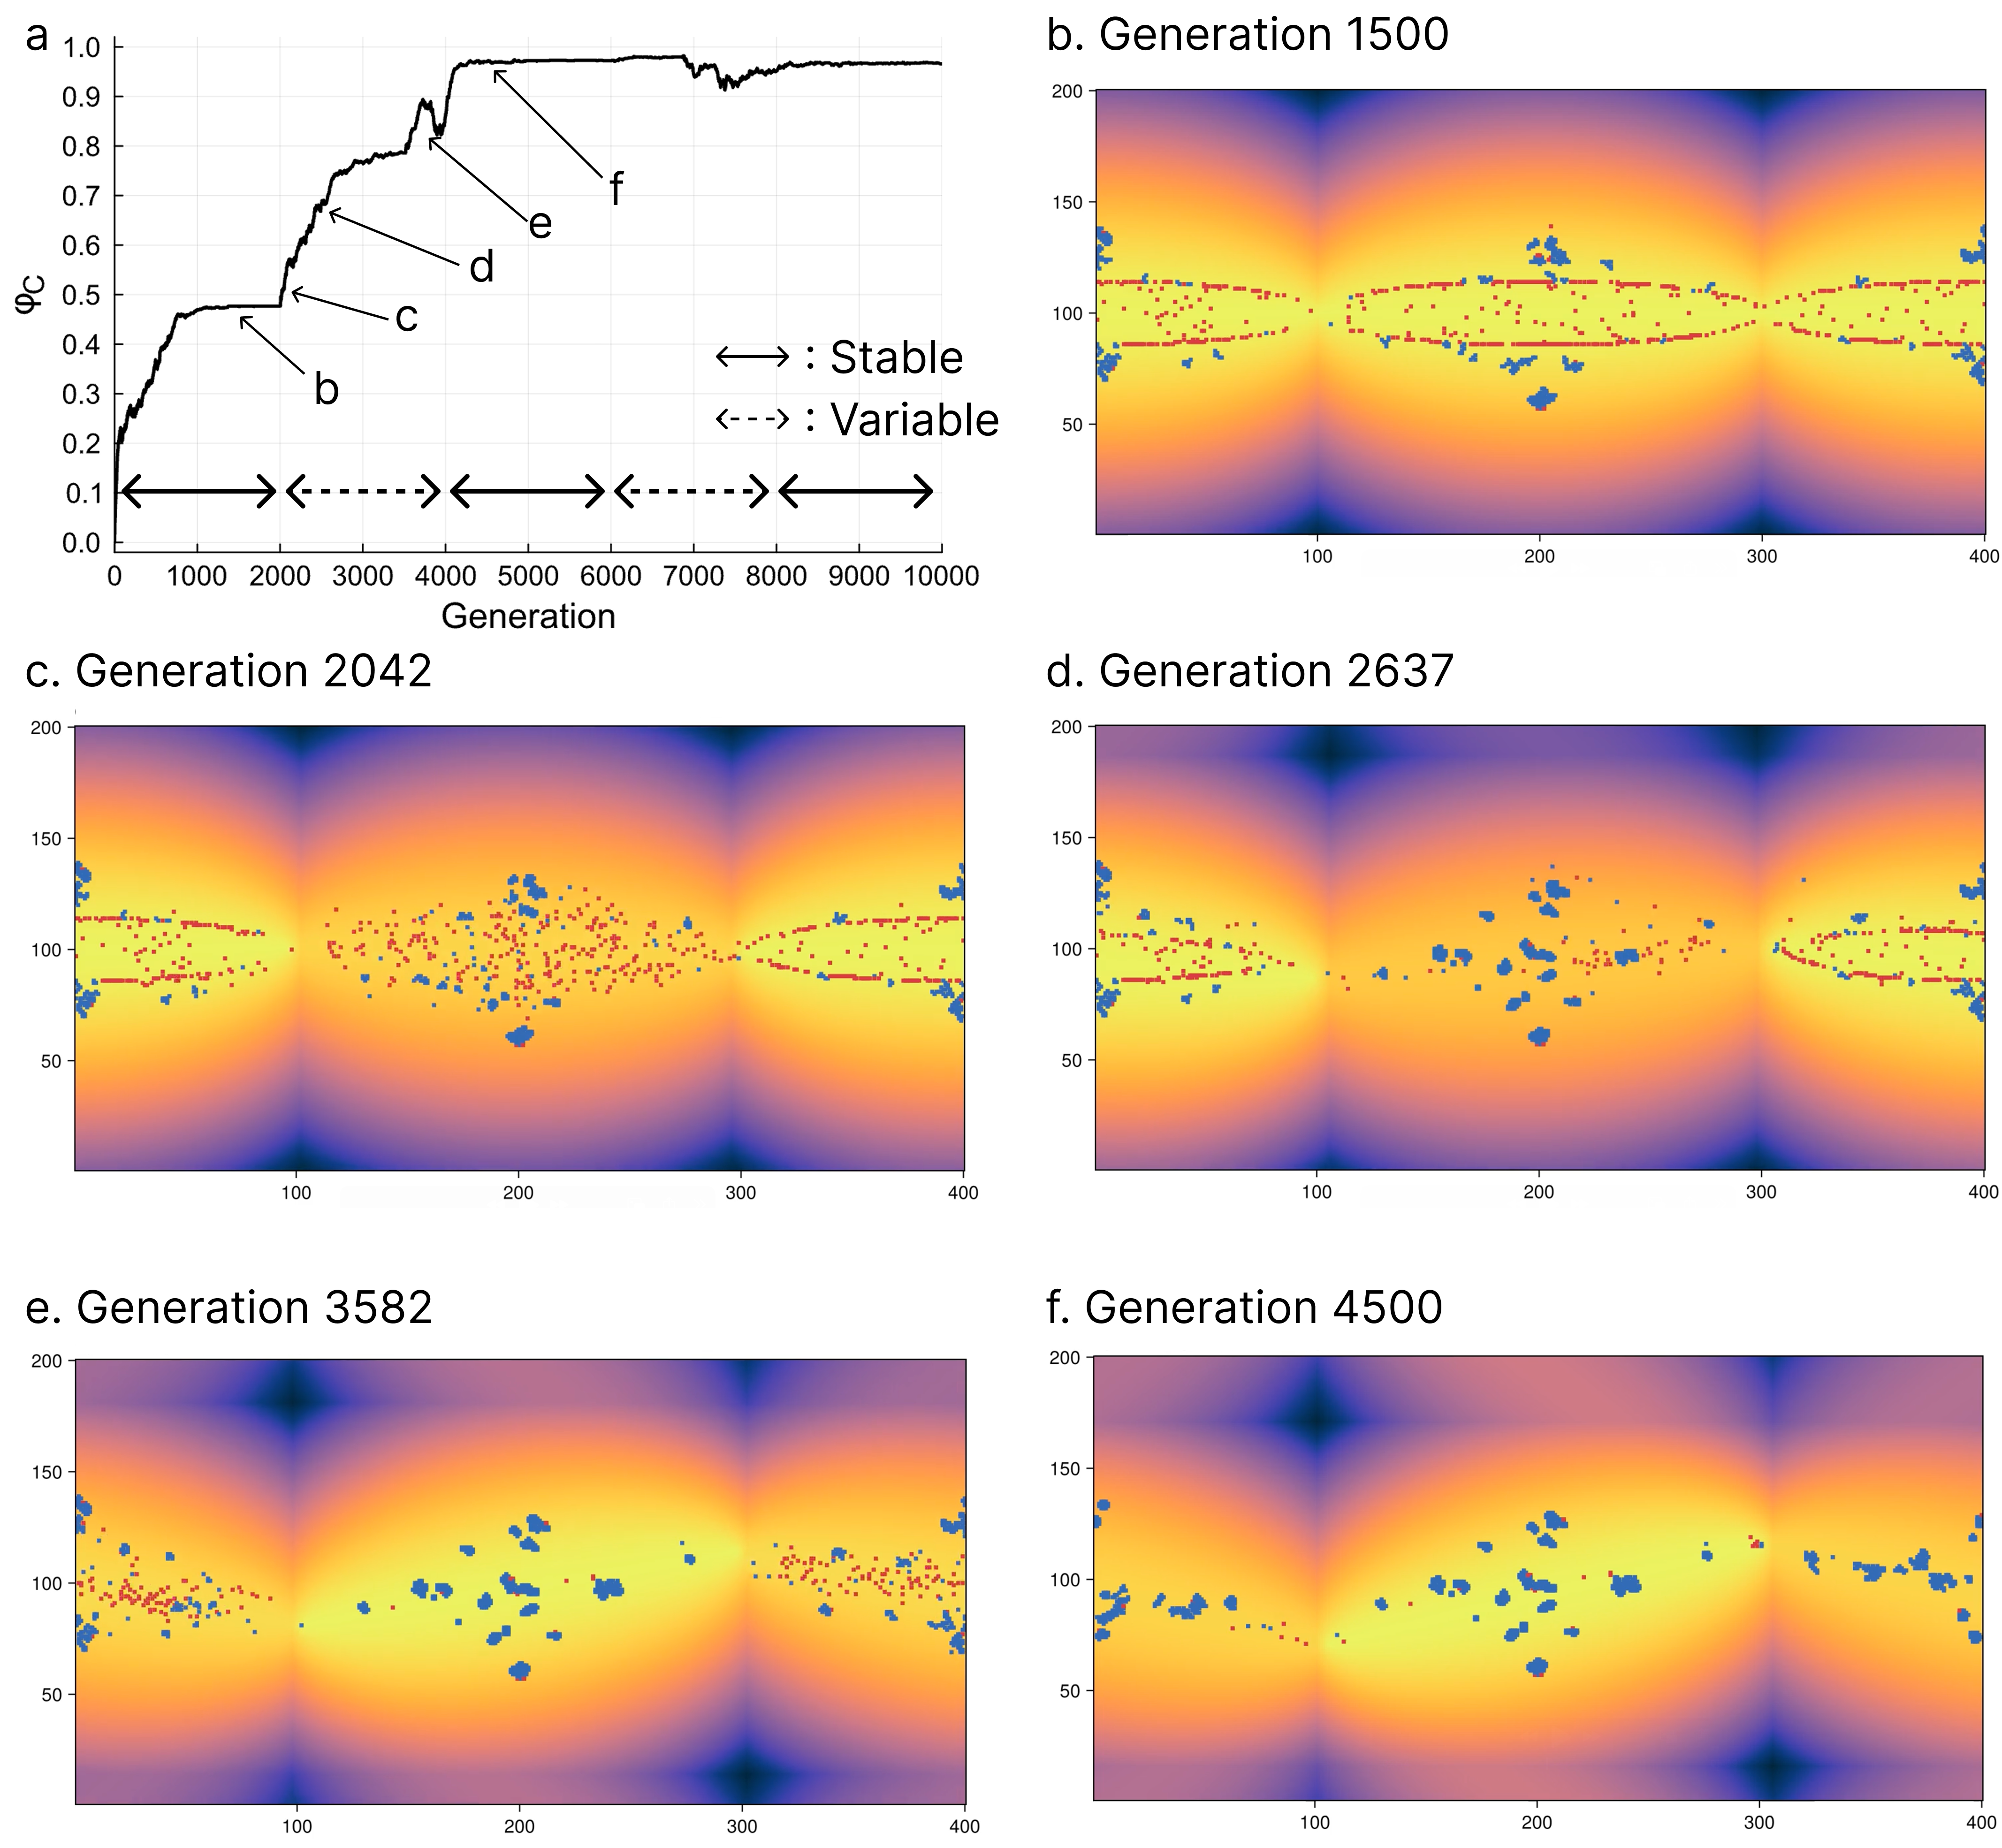
\includegraphics[width=1.0\linewidth]{figures/4/Fig3.png}
\caption[Temporal dynamics under cyclic environmental variability]{
Temporal dynamics under cyclic EV.
The figure demonstrates that EV drives cooperation by disrupting stable defector groups in resource-rich areas and facilitating the formation of multiple small cooperator groups.
(a) Cooperation rate over $10000$ generations with $p_{EV}$ alternating between stable ($p_{EV} = 0$) and variable ($p_{EV} = 0.1$) phases every $2000$ generations.
(b)--(f) Spatial snapshots at each generation.
Blue and red dots represent cooperators and defectors, respectively.
Background colors indicate the resource threshold $\theta_{x,y}$ as in Figure~\ref{fig:ev}.
Parameter settings: $N = 1000$, $\phi_C^0 = 0.0$, 2-SoR, $T = 1.2$, $S = -0.2$, $p_M = 1.0$, $p_{SoR} = 0.1$, $\mu = 0.01$.
}\label{fig:4_temporal_01_10}
\end{figure}

The observed dynamics can be understood as a three-stage process:
(i) the formation of a few large defector groups fixed in resource-rich areas,
(ii) their collapse induced by EV, and
(iii) subsequent emergence of several small cooperator groups.
Figures~\ref{fig:4_temporal_01_10}b--f show snapshots from the simulation presented in Figure~\ref{fig:4_temporal_01_10}a.
A full video showing this process is provided in the \nameref{appendix}.
In the first stable phase as shown in Figure~\ref{fig:4_temporal_01_10}b, the agents in prosperous areas have no need to cooperate or move, whereas those in less prosperous areas must cooperate or move to prosperous areas.
At the boundaries between these two areas, fixed walls are formed by defectors who do not need to change their strategies or move further.
During the next variable phase as shown in Figures~\ref{fig:4_temporal_01_10}c--e, agents located on boundaries are forced to cooperate or move due to the environmental changes, thereby leading to the collapse of the stable defector group as shown in the central area of Figure~\ref{fig:4_temporal_01_10}c.
In place of the defector group, the agents form several small cooperator groups to survive even in severe environmental conditions (Figure~\ref{fig:4_temporal_01_10}d).
Then, the same process occurs in the areas at both ends of the figure (Figures~\ref{fig:4_temporal_01_10}e and f).

In contrast, cooperation cannot evolve if the agent mobility is insufficient relative to the intensity of the EV (refer to the lower area of Figure~\ref{fig:4_key_result}),
which occurs because excessively rapid SoR movement prevents the formation of both defector structures and small cooperator groups, as shown in Figure~\ref{fig:4_temporal_01_01}.
Thus, EV and sufficient agent mobility promote cooperation by preventing fixed defector structures and encouraging the agents to form cooperator groups for survival.

\begin{figure}[!ht]
\centering
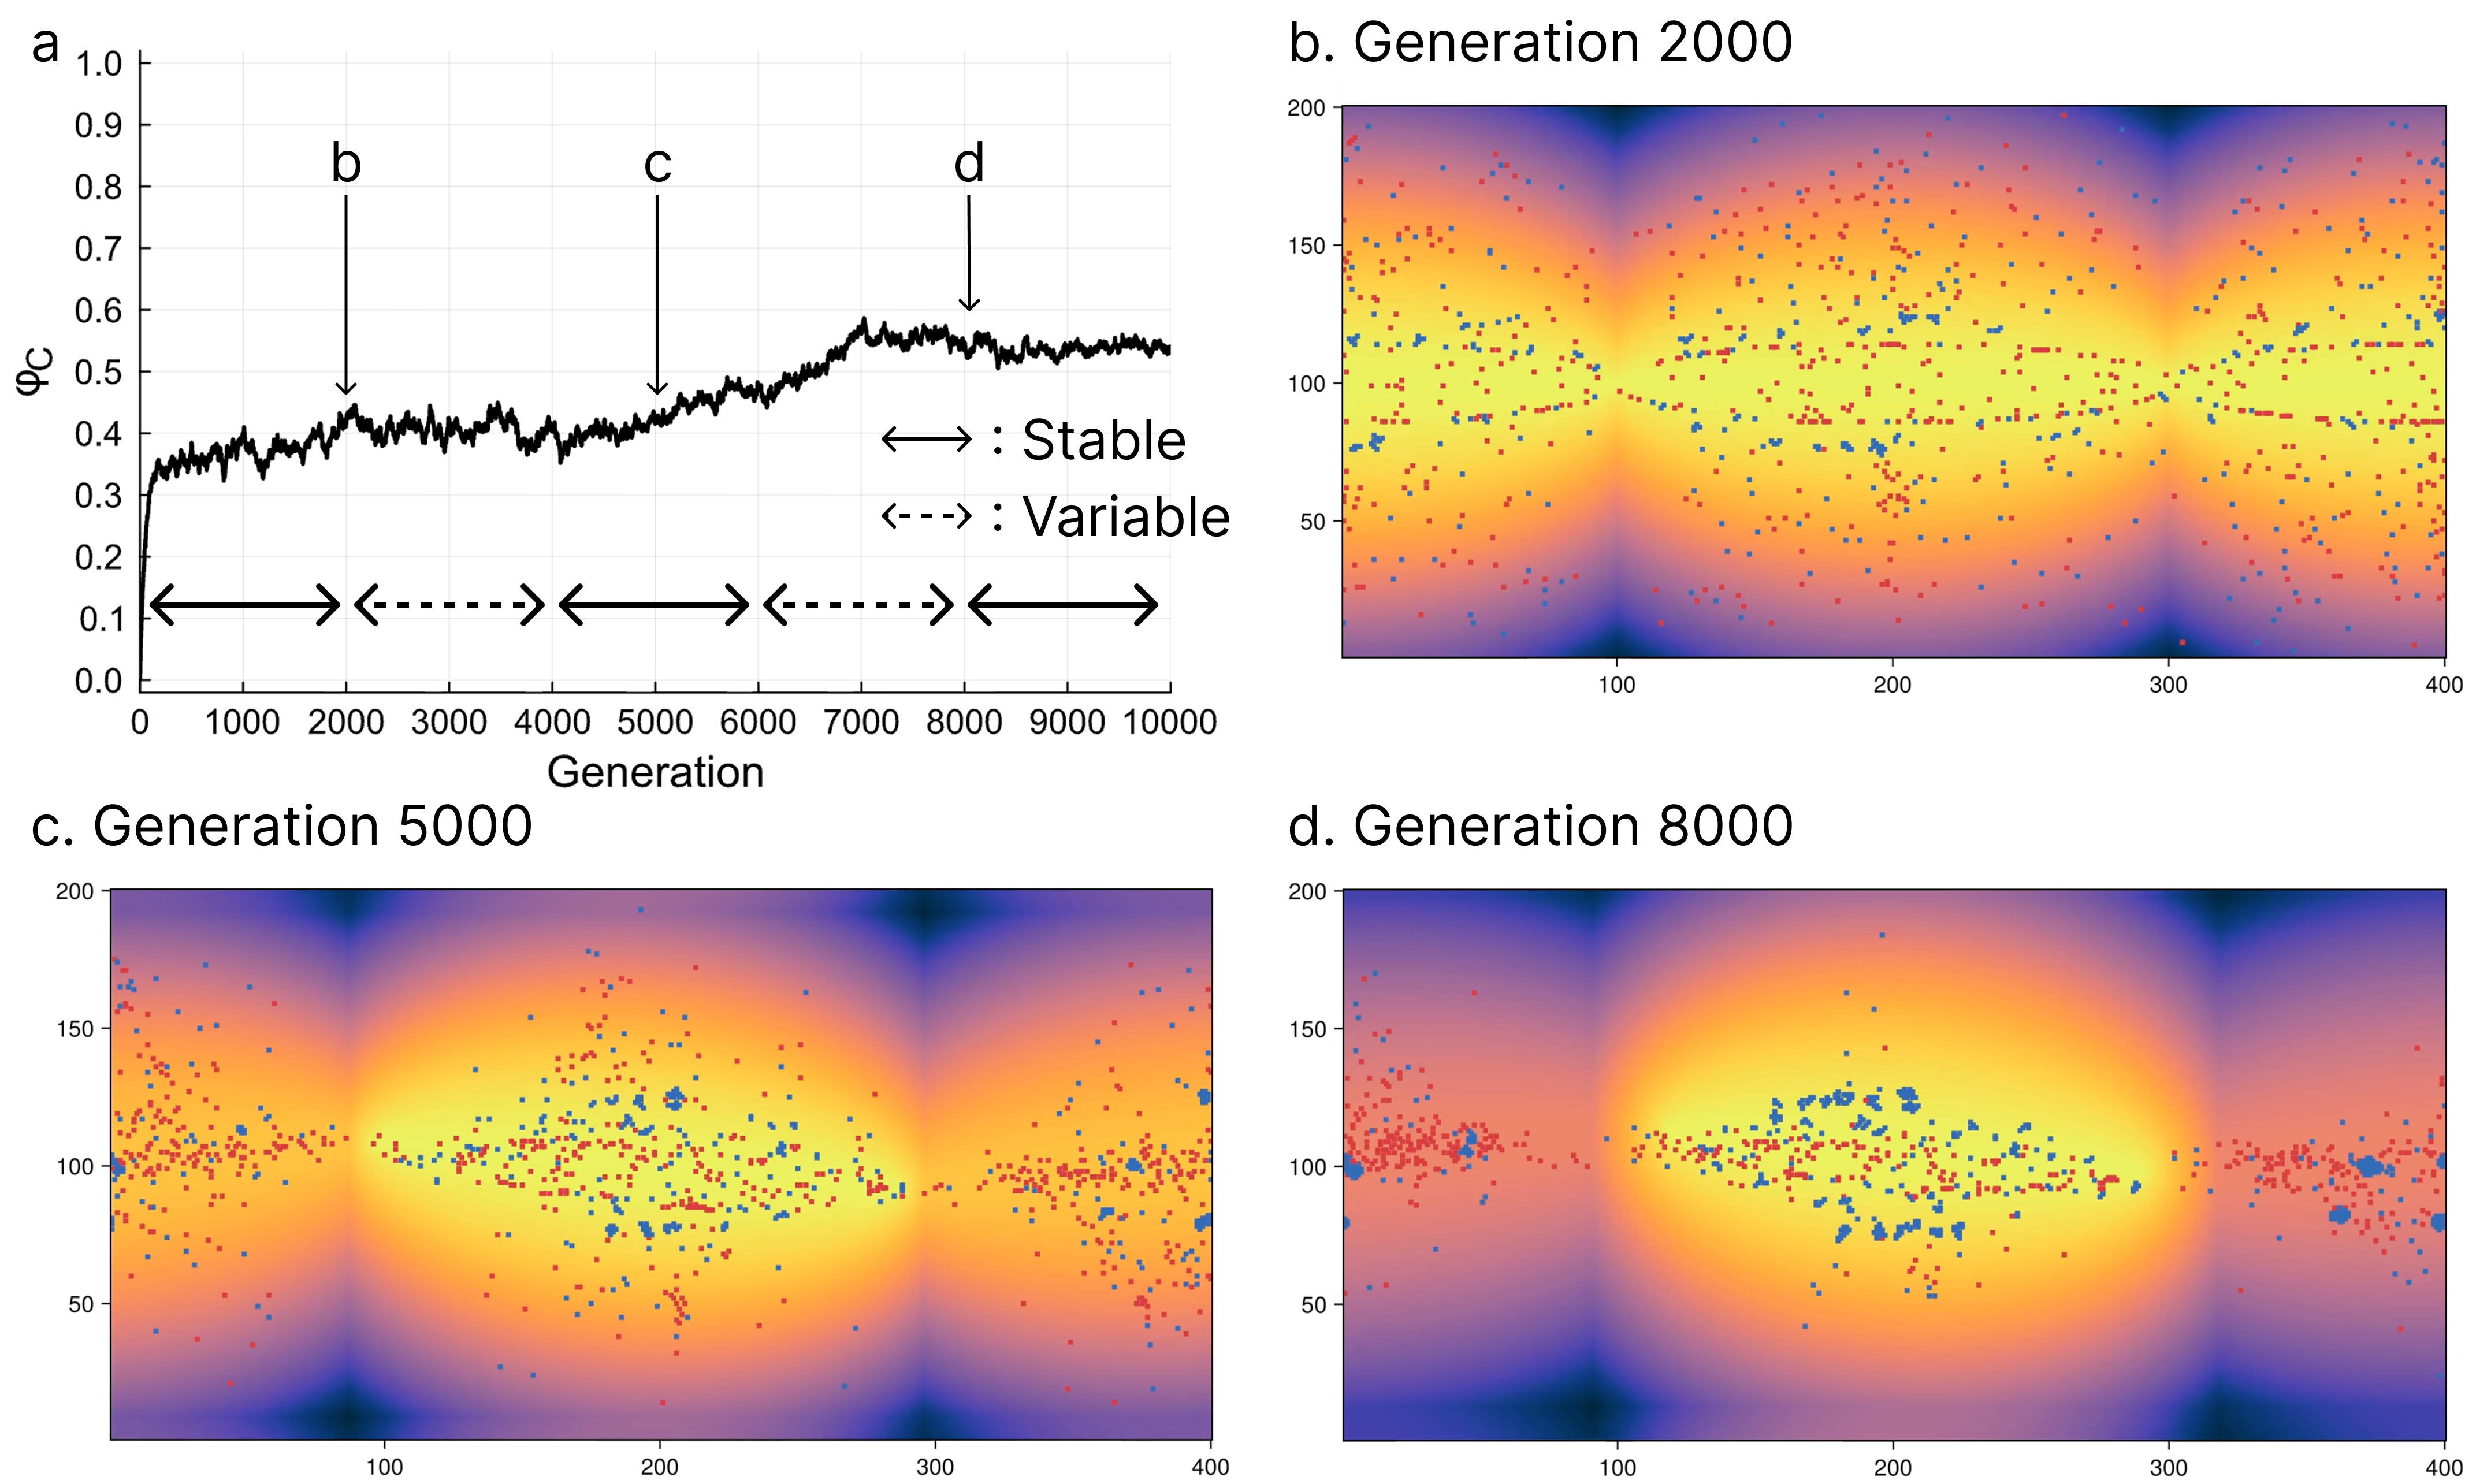
\includegraphics[width=1.0\linewidth]{figures/4/Fig4.png}
\caption[Temporal dynamics under cyclic environmental variability with low agent mobility]{
Temporal dynamics under cyclic EV with low agent mobility.
In contrast to Figure~\ref{fig:4_temporal_01_10} ($p_M = 1.0$), here lower mobility ($p_M = 0.1$) prevents agents from keeping up with the EV.
As a result, cooperation fails to evolve.
All other parameters and the interpretation of the visual elements are the same as in Figure~\ref{fig:4_temporal_01_10}.
}\label{fig:4_temporal_01_01}
\end{figure}

\subsection*{Influence of other parameters on cooperation rate}

To gain further insights into the findings presented above and assess their robustness, we investigated the effects of additional parameters, including the population size ($N$), the number of SoRs ($n_{SoR}$), the initial frequency of cooperators ($\phi_C^0$), the SoR orientation ($p_{SoR}$), the payoff parameters ($T$, $S$), and the mutation rate ($\mu$).

\subsubsection*{Population size}

Larger population size promotes cooperation to some extent, as shown in Figure~\ref{fig:4_population}, because the cooperators can more easily find other cooperators when the population size is sufficiently large.

Another notable observation is that the cooperation rates for $(p_{EV}, p_M) = (0.0, 0.1)$ (red dashed line) and $(0.1, 0.1)$ (blue dashed line) exhibit a crossover at approximately $N = 2000$.
For small populations ($N < 2000$) with low agent mobility, cooperation evolves more readily without EV.
In stable environments ($(p_{EV}, p_M) = (0.0, 0.1)$), both the defector and cooperator groups persist once established, although the formation of these groups is slow due to the low agent mobility.
In contrast, EV with low agent mobility ($(p_{EV}, p_M) = (0.1, 0.1)$) creates perpetual fluidity that prevents the formation of both structures.

Larger populations alter this relationship.
Larger populations increase the encounter rate among cooperators, which allows for the formation of cooperator groups even under EV.
In stable environments, the structures remain fixed, thereby limiting the impact of the higher encounter rate.
In contrast, the higher encounter rate in fluid environments facilitates group formation.
Thus, EV becomes advantageous for cooperation above the critical population size.

A less prominent but similar crossover occurs at approximately $N = 8000$ between $(p_{EV}, p_M) = (0.0, 0.1)$ (red dashed line) and $(p_{EV}, p_M) = (0.0, 1.0)$ (red solid line).
This crossover reflects the spatial constraints of the defector groups in stable environments ($p_{EV} = 0$).
For $N \lesssim 8000$, high mobility ($p_M = 1.0$) allows more agents to reach the resource-rich areas where cooperation is not required.
In contrast, low mobility ($p_M = 0.1$) keeps the agents in peripheral areas where cooperation is required for survival.

However, larger populations ($N \gtrsim 8000$) exhibit three nested zones:
central rich areas, where cooperation is not required;
surrounding moderate areas, where the agents can survive through cooperation; and
the most peripheral harsh areas, where agents cannot survive even with cooperation because the resource threshold exceeds what can be provided through cooperation.
Under these conditions, high mobility allows the agents to escape from the harsh areas to the moderate cooperative areas, whereas low mobility traps the agents in the harsh areas.
In addition, the central rich areas have already reached their physical capacity due to the large population;
thus, further population increases have no effect in these areas.
Consequently, the effect of mobility on the cooperation rate ($\phi_C$) reverses as the population size increases.

\begin{figure}[!ht]
\centering
\includegraphics[width=0.7\linewidth]{figures/4/Fig5.png}
\caption[Influence of population size ($N$) on cooperation rate ($\phi_C$)]{
Influence of population size ($N$) on cooperation rate ($\phi_C$).
The figure shows two crossovers: at $N \approx 2000$ between $(p_{EV}, p_M) = (0.0, 0.1)$ (red dashed) and $(0.1, 0.1)$ (blue dashed), and at $N \approx 8000$ between $(0.0, 0.1)$ (red dashed) and $(0.0, 1.0)$ (red solid).
These crossovers reflect how population size alters the relative benefits of EV and mobility through changes in cooperator encounter rates and spatial resource distribution.
Parameter settings: $\phi_C^0 = 0.0$, 2-SoR, $T = 1.2$, $S = -0.2$, $p_{SoR} = 0.1$, $\mu = 0.01$.
The results for $N = 32000$ are omitted because they exhibited negligible differences from $N = 16000$.
}\label{fig:4_population}
\end{figure}

\subsubsection*{Number of SoRs and initial cooperation rate}

Both the number of SoRs ($n_{SoR}$) and the initial frequency of cooperators ($\phi_C^0$) have a significant influence on the results.
While the 2-SoR configuration forms large band-shaped defector groups (Figure~\ref{fig:4_temporal_01_10}b), the 1-SoR configuration only forms a small, circular resource-rich area (Figure~\ref{fig:4_1sor}b).
When a large defector group collapses and is replaced by small cooperator groups, as observed with the 2-SoR setting, the impact on the overall system is substantial.
In contrast, under the 1-SoR setting, when a small defector group undergoes the same replacement, the effect is less conspicuous than in the 2-SoR setting (Figure~\ref{fig:4_1sor}a).
In terms of $\phi_C^0$, initiation with no cooperators ($\phi_C^0 = 0$) in the 2-SoR configuration results in large defector groups, whereas intermediate or full cooperation ($\phi_C^0 = 0.5$ or $1$) maintains the large structure but with a higher cooperator frequency within it (Figure~\ref{fig:4_phiC0}).
Consequently, these conditions mask the significant effects of defector group collapse and cooperator group formation observed in Subsection~\ref{sec:4_key_results}.

We also confirmed that changing the distance metric from Euclidean to the Chebyshev or Manhattan distance alters the size and shape of the groups, thereby affecting the results.
However, these effects are primarily attributed to differences in the group size rather than the shape.
Thus, comparisons among these distance metrics can be interpreted as theoretically equivalent to the comparison between the 1-SoR and 2-SoR settings.
Essentially, the formation of large defector groups in stable environments is the critical prerequisite for the results described in Subsection~\ref{sec:4_key_results}.

\begin{figure}[!ht]
\centering
\includegraphics[width=1.0\linewidth]{figures/4/Fig6.png}
\caption[Temporal dynamics under cyclic environmental variability in the 1-SoR configuration]{
Temporal dynamics under cyclic EV in the 1-SoR configuration.
The figure shows that the 1-SoR configuration forms only a small circular resource-rich area, resulting in a less pronounced impact of defector group collapse on overall cooperation levels compared to Figure~\ref{fig:4_temporal_01_10} (2-SoR).
All other parameters and the interpretation of the visual elements are the same as in Figure~\ref{fig:4_temporal_01_10}.
}\label{fig:4_1sor}
\end{figure}

\begin{figure}[!ht]
\centering
\includegraphics[width=1.0\linewidth]{figures/4/Fig7.png}
\caption[Central resource-rich areas under $\phi_C^0 = 0.5$ or $1.0$]{
Central resource-rich areas under $\phi_C^0 = 0.5$ or $1.0$.
The figure shows that higher initial cooperation rates maintain larger cooperative structures in resource-rich areas, masking the effects of defector group collapse and cooperator group formation observed with $\phi_C^0 = 0.0$.
All parameters (except $\phi_C^0$) and the interpretation of the visual elements are the same as in Figure~\ref{fig:4_temporal_01_10}.
}\label{fig:4_phiC0}
\end{figure}

\subsubsection*{SoR orientation}

SoR orientation ($p_{SoR}$) noticeably influences the cooperation rate (Figure~\ref{fig:4_sor_orientation}).
Increasing $p_{SoR}$ from $0$ to $0.1$ improves cooperation rates by approximately 20\%--40\% if $p_{EV} > 0$.
However, further increases in $p_{SoR}$ beyond $0.2$ reduce the cooperation rate.
This reduction occurs because excessive $p_{SoR}$ increases the likelihood of agent collisions, which in turn hinders effective migration.
These findings suggest that some randomness in the agent mobility is required to maintain a high level of cooperation.

\begin{figure}[!ht]
\centering
\includegraphics[width=0.6\linewidth]{figures/4/Fig8.png}
\caption[Influence of SoR orientation ($p_{SoR}$) on the cooperation rate ($\phi_C$)]{
Influence of SoR orientation ($p_{SoR}$) on the cooperation rate ($\phi_C$).
The figure shows that moderate SoR orientation ($p_{SoR} \approx 0.1$) maximally promotes cooperation, while excessive $p_{SoR}$ reduces cooperation due to increased agent collisions that hinder effective migration.
Parameter settings: $N = 1000$, $\phi_C^0 = 0.0$, 2-SoR, $p_M = 1.0$, $T = 1.2$, $S = -0.2$, $\mu = 0.01$.
}\label{fig:4_sor_orientation}
\end{figure}

\subsubsection*{Payoff parameters and mutation rate}

We also investigated the effects of varying the values of the payoff parameters $(T, S)$ across several game structures and the mutation rate $\mu$ (including $\mu = 0$ and $\mu = 0.01$).
While these variations did not yield qualitatively new insights, they confirmed the robustness of the observed patterns.
For completeness, the corresponding results are provided in the \nameref{appendix}.

\section{Summary}\label{sec:4_summary}

In this chapter, we examined the joint effects of EV and agent mobility on the evolution of cooperation to understand the causal dynamics of these factors in spatially structured populations.
The model incorporates unpredictable EV by implementing SoRs that move randomly across a 2D space, generating dynamic spatial heterogeneity in resource availability.
Agents accumulate resources through cooperative or competitive interactions, and the agents with lower resource levels are more likely to migrate to neighboring cells and update their strategies.
With this model, we identified three key findings.
First, with sufficient agent mobility, even modest EV promotes cooperation; however, further variability does not enhance cooperation.
Second, with any level of EV, agent mobility promotes cooperation.
Third, these effects occur because EV disrupts a few large stable defector groups that form in resource-rich areas, and agent mobility effectively enables the formation of numerous small cooperator groups at those sites.

The next chapter, Chapter~\ref{ch:5_conclusion}, synthesizes and compares the findings from all three models to identify common mechanisms and discuss the broader implications for understanding the evolution of cooperation under EV.